\documentclass{article}


\usepackage{PRIMEarxiv}

\usepackage[utf8]{inputenc} % allow utf-8 input
\usepackage[T1]{fontenc}    % use 8-bit T1 fonts
\usepackage{hyperref}       % hyperlinks
\usepackage{url}            % simple URL typesetting
\usepackage{booktabs}       % professional-quality tables
\usepackage{amsfonts}       % blackboard math symbols
\usepackage{nicefrac}       % compact symbols for 1/2, etc.
\usepackage{microtype}      % microtypography
\usepackage{lipsum}
\usepackage{fancyhdr}       % header
\usepackage{graphicx}       % graphics
\graphicspath{{media/}}     % organize your images and other figures under media/ folder
\usepackage{wrapfig}
\usepackage{subcaption}

\graphicspath{{images/}}
%Header
\pagestyle{fancy}
\thispagestyle{empty}
\rhead{ \textit{ }} 

% Update your Headers here

% \fancyhead[RE]{Firstauthor and Secondauthor} % Firstauthor et al. if more than 2 - must use \documentclass[twoside]{article}



  
%% Title
\title{Assignment : Predicting Meter
%%%% Cite as
%%%% Update your official citation here when published 
}

\author{
  Jan Grielens \\
  UAntwerpen \\
  Master Digital Text Analysis\\
  Machine Learning\\
  2023-2024 \\
}


\begin{document}
\maketitle


\begin{abstract}
This paper investigates the application of machine learning methods, comparing neural networks and traditional approaches, to predict the meter in poetry. Analyzing rhythm patterns in verses, it explores both rule-based and neural network models for classifying poetic meters. The study demonstrates the feasibility of using rhythmic encoded patterns for meter prediction and suggests potential for future research in direct meter detection from spoken verses
\end{abstract}





\section{Introduction}

In language, music, and poetry, rhythmic features play a crucial role in understanding. This area has been under investigation since Logan's work in 1988 \cite{LoganRythm}. Historically, poets adhered to traditional and strict formats. However, in today's postmodern era, there is a trend towards exploring novel ways to deviate from these conventions. The learning, deciphering, and identification of these patterns, including meter and foot, remain integral to the study and practice of poetry.
Recent developments in natural language processing (NLP) have led to research exploring new NLP approaches. The transition from spoken sound to written word often results in the loss of rhythmic information. A sentence can be viewed as a combination of phonetic syllables, stressed or unstressed. A 'foot' comprises two or three parts, stressed (s) or unstressed (w), leading to 12 possible combinations, known as 'feet', which include 4 bigram and 8 trigram combinations. Traditionally, English poetry utilizes seven of these combinations.
\begin{table}[h!]
    \centering
    \caption{Seven Poetic Feet and Their Stresses}
    \label{tab:poetic_feet_stresses}
    \begin{tabular}{|c|c|c|c|c|c|c|c|}
    \hline
    \textbf{Category} & \multicolumn{7}{c|}{Poetic Feet and Stresses} \\ \hline
    \textbf{Names}    & Iamb & Trochee & Dactyl & Anapest & Pyrrhic & Amphibrach & Spondee \\ \hline
    \textbf{Stresses} & ws   & sw     & sww    & wws     & ww      & wsw        & ss      \\ \hline
    \end{tabular} 
\end{table}

Meters then are  described as a repetition, from one to eight, of a specific feet. If the foot is repeated once, then the verse is monometer, twice then it is a dimeter verse, until the octameter, eight repetitions of the same foot.

We will investigate both neural network approach and traditional machine learning approaches to their feasibility in this context.




 


\section{Related research}
\label{sec:headings}

Until recently, computational approaches to verse analysis were predominantly rule-based, relying on phonetic dictionaries and a set of rules for phonological parsing and generating metrical patterns. Prosodic\footnote{\url{https://github.com/quadrismegistus/prosodic}}, based on the CMU pronunciation dictionary, also utilizes the Text-to-Speech engine 'espeak' for voicing unknown words to identify their phonetic signatures. Extensions of Prosodic, such as Pronouncing\footnote{\url{https://github.com/aparrish/pronouncingpy}}, Erato\footnote{\url{https://github.com/manexagirrezabal/erato}}, and Poesy\footnote{\url{https://github.com/quadrismegistus/poesy}}, also employ the CMU pronunciation dictionary. In contrast, Rantanplan \cite{Rosa2020RantanplanFA}, initially developed for Spanish, utilizes SpaCy. ZeuScansion \cite{agirrezabal-etal-2013-zeuscansion} employs finite-state technology for metrical scansion, while Metricalizer  is a rule-based tool for metrical annotation in German.\footnote{\url{https://www.metricalizer.de/en/metrikanalyse/}}

Agirrezabal \cite{AgirrezabalLTSM} employed LSTM methods to predict the metrical patterns in lines of verse, achieving a per-line accuracy of 61.39\% for English. Yousef et al.\cite{Yousef2019LearningMetersArabicEnglish-arxiv} adopted a distinct approach by using featureless, character-based inputs in different RNN networks, reporting an overall accuracy of 82.31\% for English. The methodology of Transformers was also explored by de la Rosa et al. \cite{Delarosa2021Transformers}, which provided a baseline for both rule-based and neural network approaches \cite{Alberti}.
\begin{figure}[h!]
 \centering
 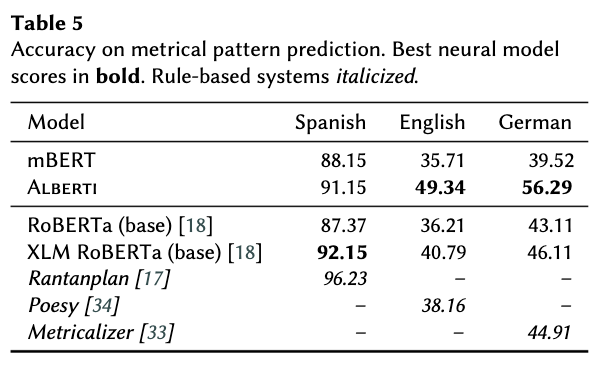
\includegraphics[width=0.5\textwidth, height=5cm]{images/alberti.png}
 \caption{Baseline for Accuracy of rule-based and alternative methods}
\end{figure}

\section{Experimental design}
\label{sec:headings}



\subsection{Data}

The English dataset comprises 199,002 verses. Each verse is categorized into one of four meters: Iambic, Trochee, Dactyl, and Anapaestic. The dataset is predominantly Iambic, with 186,809 Iambic verses, followed by 5,418 Trochee, 5,378 Anapaestic, and 1,397 Dactyl verses \textbackslash{}cite\{PCD2018\}. For our analysis, we utilized the Down-sampled English PCD, which includes 17,743 verses. \href{https://www.kaggle.com/datasets/mohamedkhaledelsafty/english-poem-comprehensive-dataset-apcd?select=Down-sampled+English+PCD.csv}{}

\begin{figure}[h!] 
\begin{subfigure}{0.5\textwidth}
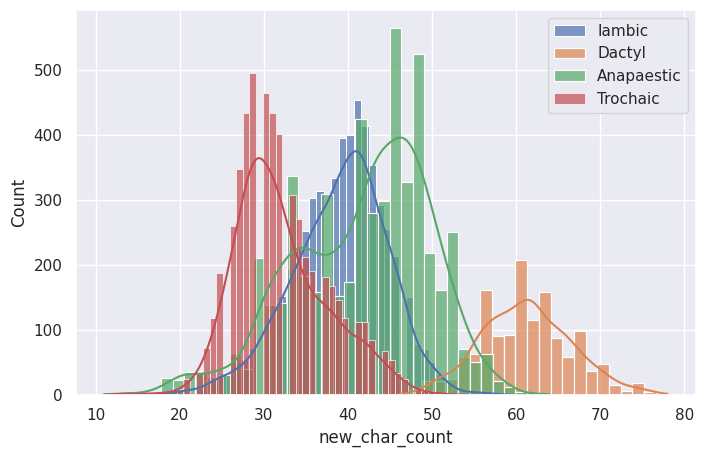
\includegraphics[width=0.9\linewidth, height=6cm]{images/word_char.png} 
\centering
\caption{Char count per Meter}
\label{fig:sub}
\end{subfigure}
\begin{subfigure}{0.5\textwidth}
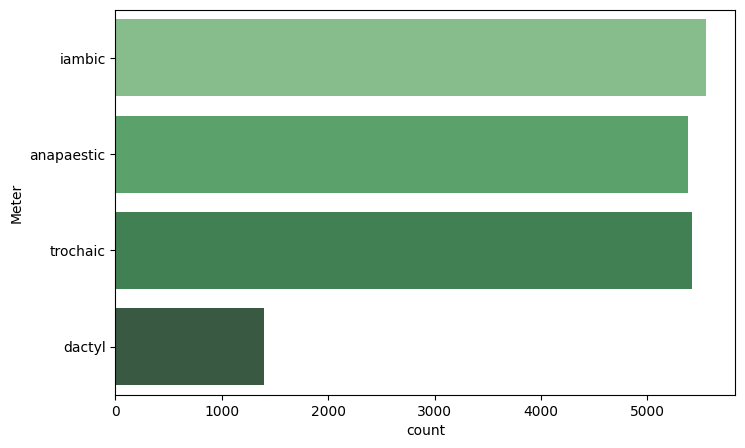
\includegraphics[width=0.9\linewidth, height=6cm]{images/D-EPCD.png} 
\centering
\caption{Distribution per Meter}
\label{fig:distribution}
\end{subfigure}
    
\end{figure}

\subsection{Tokenizing data}

We experimented with various code bases (Prosodic, Pronouncing, Scansion, and Erato) to translate verses into stress patterns (strings). Owing to its ease of use and comprehensive documentation, we selected Prosodic for this task. Each verse in the dataset was parsed into a string of 'w's and 's's, representing the stress patterns. Subsequently, the dataset underwent further preprocessing and was saved to our local system.
\begin{figure}[h!]
 \centering
 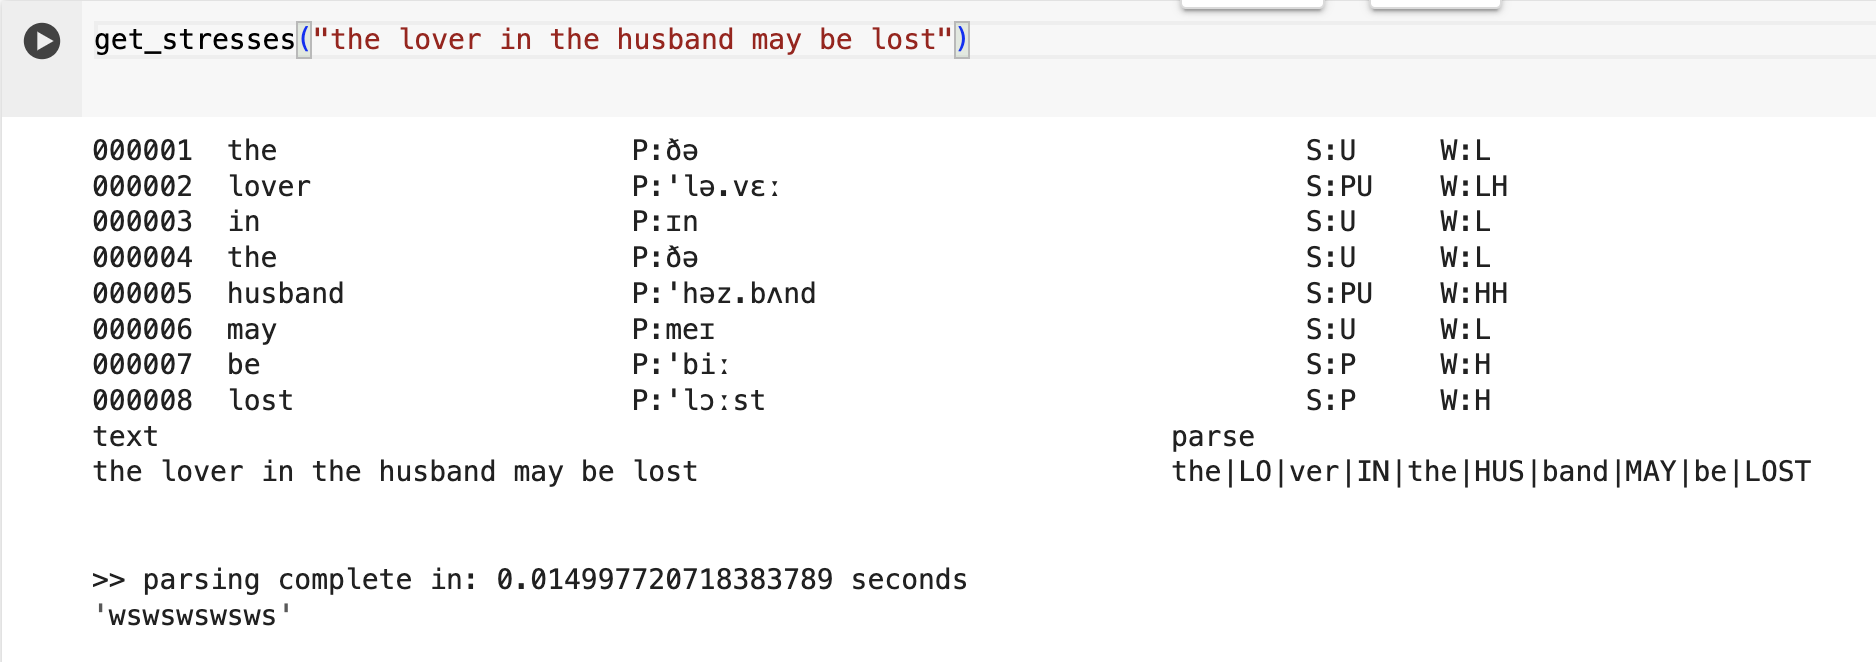
\includegraphics[width=0.7\textwidth]{images/stressed_line.png}
 \caption{Calculated stress pattern by Prosodic }
\end{figure}
The dataset was then further preprocessed and saved to our local system.


\subsection{Methods and experiments}

We aimed to evaluate the feasibility of two methods for predicting one of four meters from a string, such as 'wswswswsw'. These methods align with the bigram-trigram approach traditionally used in English meter analysis. The preprocessed data was divided into a 60/20/20 split for training, validation, and testing.

The first model is XGBoost, a tree-based algorithm. It employs a level-wise strategy, scanning across gradient values and using these sums to evaluate the quality of splits at every potential point in the training set. For our classification task, we used \verb|mlogloss|, a metric designed for multiclass classification problems and comparable to the categorical crossentropy loss. We adapted the dataset to meet the specific requirements of the XGBClassifier and applied a character-based CountVectorizer. A grid search was conducted with parameters: 'ngram range': [(1, 1), (2, 2), (1, 2), (\textbf{2, 3})], 'depth': [5, \textbf{7}], 'estimators': [100, \textbf{200}], and 'learning rate': [0.01, \textbf{0.1}], with the best parameters in bold. We produced a confusion matrix, a classification-precision report, and calculated the Mean Squared Error (MSE) and Mean Absolute Error (MAE). The tree structure utilized 10 features ['ss', 'ssw', '\textbf{sw}', 'sws', '\textbf{sww}', '\textbf{ws}', '\textbf{wss}', 'wsw', 'ww', 'wws'], with the bolded features corresponding to our four meters.

The second model is a convolution model applied to text by Kim. \cite{kim-2014-convolutional}

\begin{figure}[h!]
 \centering
 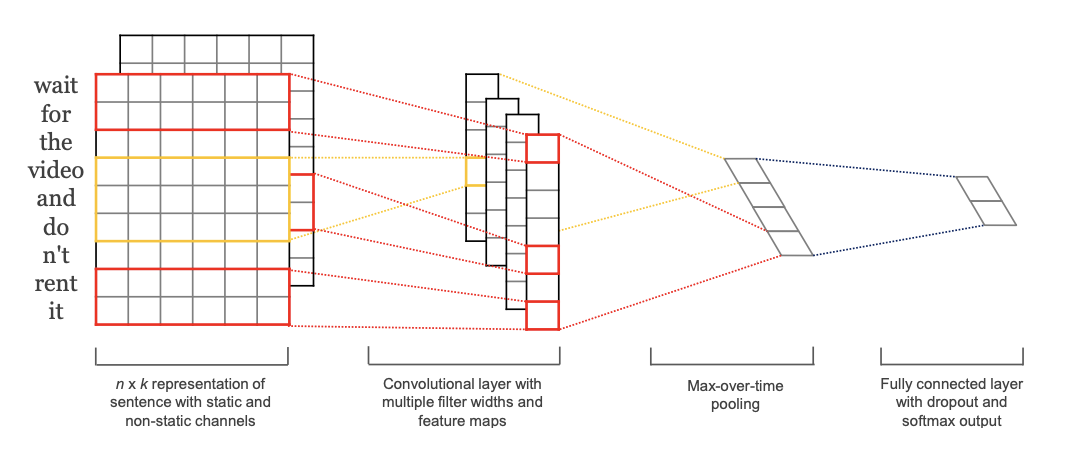
\includegraphics[width=0.7\textwidth]{images/koon.png}
 \caption{Convolution Neural Network for Sentence Classification  }
\end{figure}

We adjusted this approach to one string of 'wswssswsws', padded to the maximum length because the convolution needs fixed length vectors. Three convolution layers were used with respective 1, 2 and 3 size kernels. Then a GlobalMaxPooling layer and a Dense layer with SoftMax. The \verb|CategoricalCrossentropy| was used as a loss function applicable for our multiclass classification problems.  This function heavily penalizes discrepancies between true labels (one-hot encoded) and predicted probabilities, applying milder penalties for correct predictions. For optimization, we chose Stochastic Gradient Descent (SGD) with a learning rate of 0.01 and momentum of 0.9. The training was conducted over 10 epochs.
        
\subsection{System}
Jupyter Notebook in Google Colab with a  V100 runtime. Coding was done with the assistance of ChatGPT 4.0,  used for debugging, explaining code and code generation. 


\section{Results}

Our main focus was determining the feasibility of our approach. The  XGBClassifier performed with 76.00 accuracy better than the 1DConvolution (50.09 ) and second best in comparison with the rest. The XGBClassifier model has f1-score \ref{fig:addendum_xclass}between 0.72 and 0.78 with 0.98 for the Dactyl meter (sww). The 1DConvolution \ref{fig:addendum_cclass} has a low f1-score (0.22) for the Trochaic meter (sw). 

% Adding the table environment
\begin{table}[ht]
    \centering
    \begin{tabular}{ |p{5cm}|c| }
    \hline
    \multicolumn{2}{|c|}{\textbf{Comparison with Baseline}} \\
    \hline
    \textbf{Model} & \textbf{Accuracy \%}  \\
    \hline
    & \\
    Youssef: RNN  & 82.31  \\
    \textbf{Model 1: XGBClass} & \textbf{76.00}  \\
    Agirrezabal: LSTM  & 61.39  \\
  
    \textbf{Model 2: conv1D} & \textbf{50.09}   \\
    ALBERTI: Transformer & 49.34\\
    Poesy: Rule-based &  38.16  \\
   & \\
    \hline
    \end{tabular}
    \vspace{5pt}
    \caption{Baseline comparison ranked}
    \label{tab:comparison}
\end{table}


\section{Conclusion}
The current results show that on it is feasible to predict meter of verses on the basis of a rhythmic encoded pattern. We used a hybrid approach using existing methods. The 40-80 \% accuracy indicates that there is room for more research. A interesting avenue for research could be to go from spoken verses directly to meter detection. 

%Bibliography
\bibliographystyle{unsrt}  
\bibliography{references}  

\clearpage
\vspace*{4pt} % Add a little vertical space for aesthetics
\hrule 
\vspace{2pt} % Space between the rule and the title

% Centering the Addendum title manually
\begin{center}
\Large \textbf*{Addendum}
\label{sec:addendum}
\end{center}

\vspace{2pt} % Space between the title and the rule
\hrule 
\vspace{4pt} % Space after the rule


\subsection*{Mode 1: XGBClassifier}



\begin{figure}[h!] 
\begin{subfigure}{0.5\textwidth}
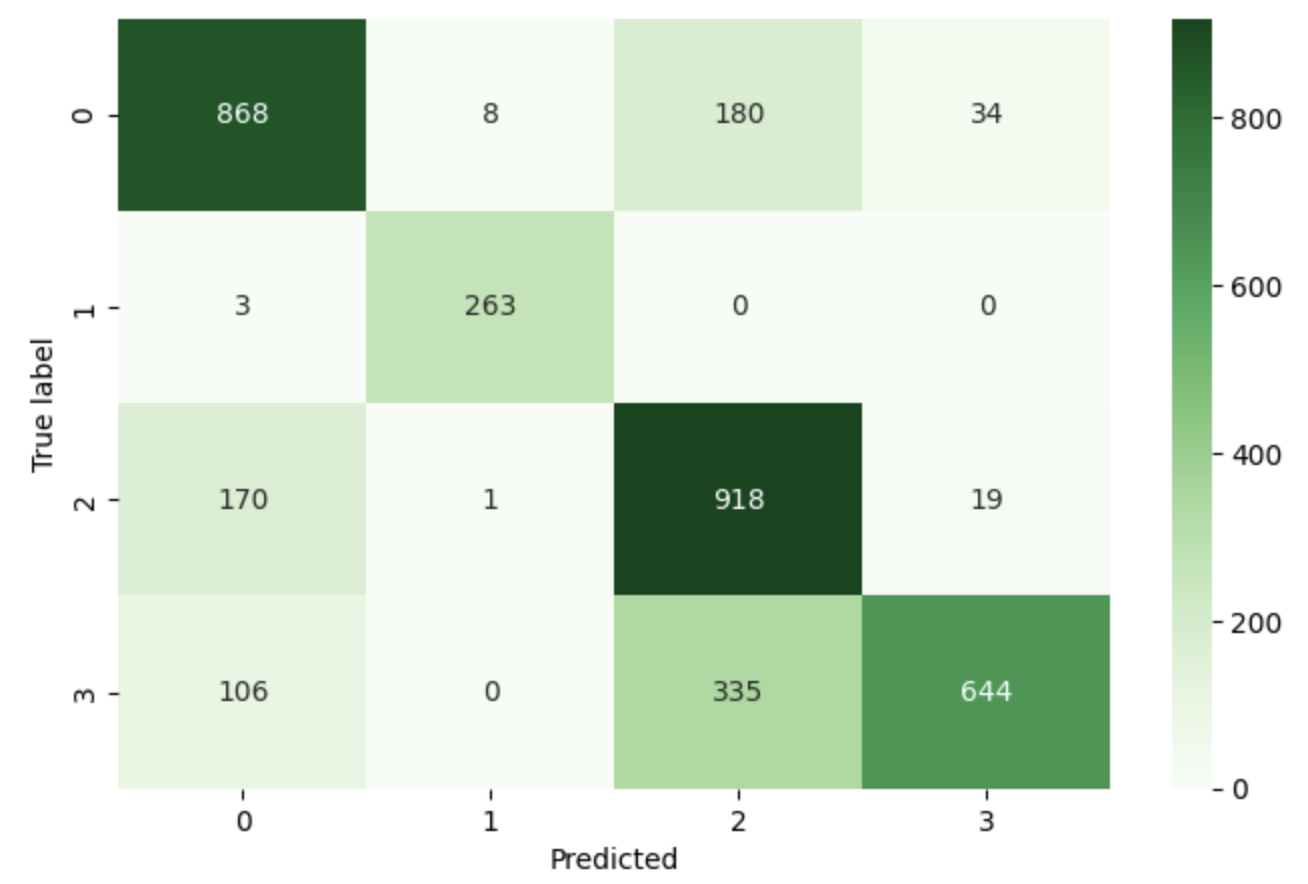
\includegraphics[width=0.9\linewidth, height=6cm]{images/XGBC_f.png} 
\centering
\caption{Confusionmatrix}
\label{fig:addendum_xcon}
\end{subfigure}
\begin{subfigure}{0.5\textwidth}
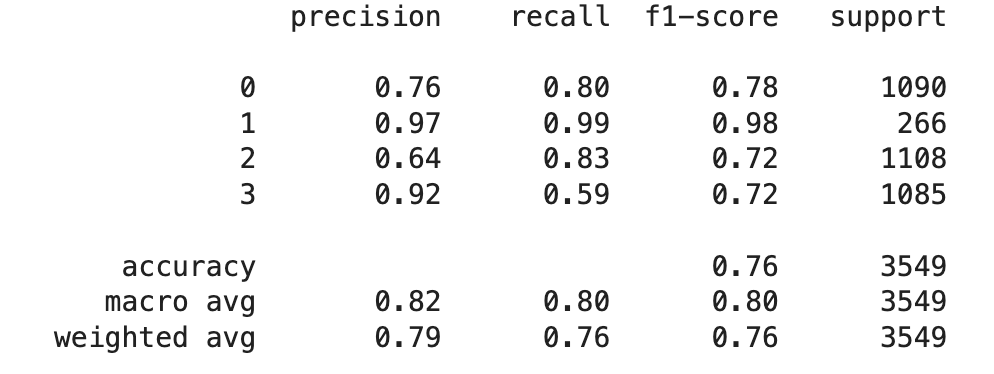
\includegraphics[width=0.9\linewidth, height=6cm]{images/XGBC_af.png} 
\centering
\caption{Classification report}
\label{fig:addendum_xclass}
\end{subfigure}
    
\end{figure}
\subsection*{Model 2: 1DConvolution}
\begin{figure}[h!] 
\begin{subfigure}{0.5\textwidth}
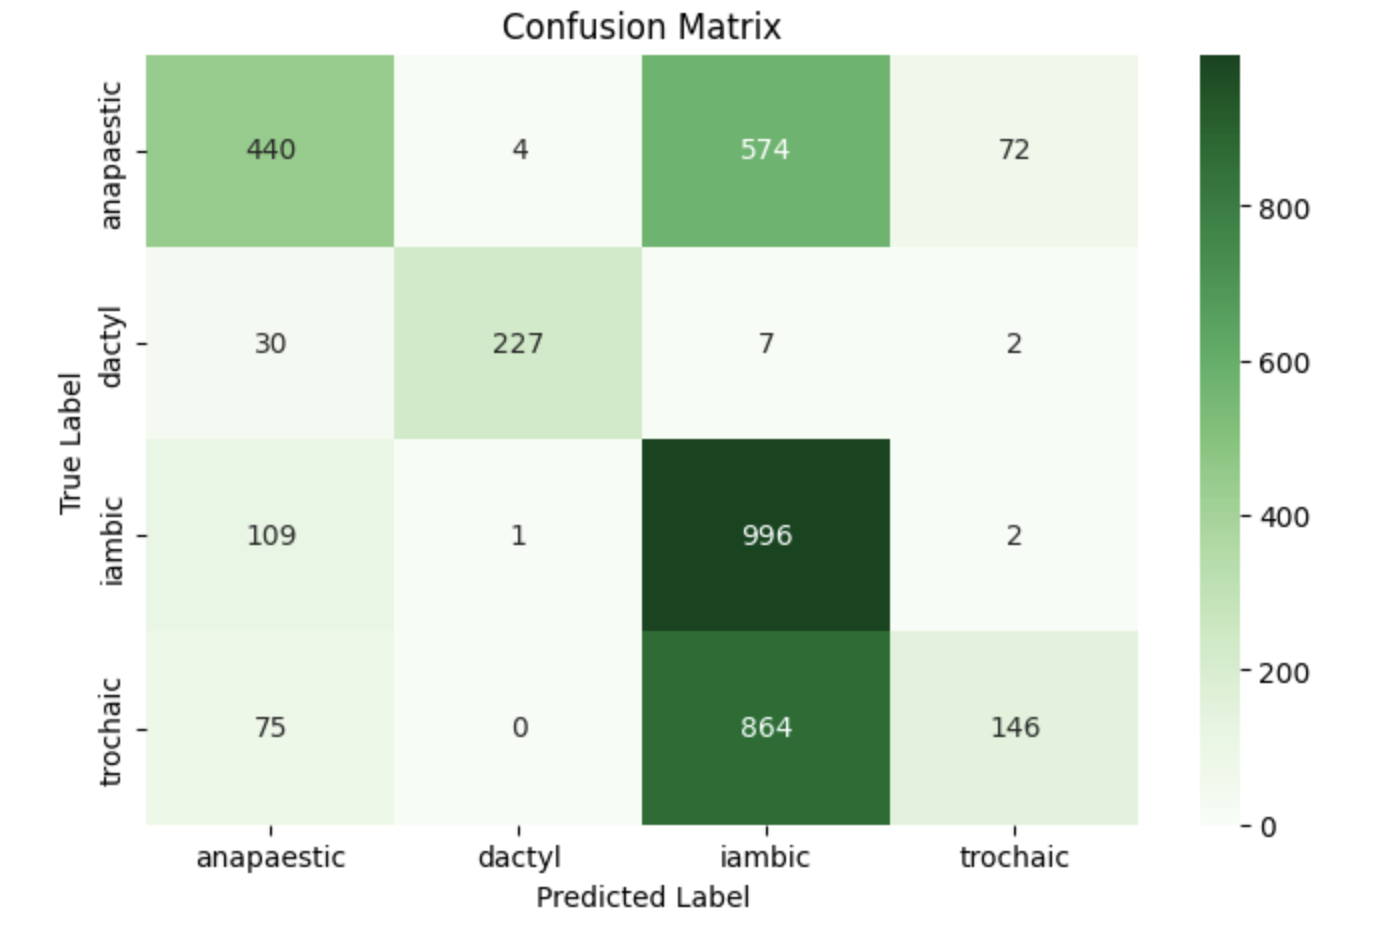
\includegraphics[width=0.9\linewidth, height=6cm]{images/1DCONV_f.png} 
\centering
\caption{Confusionmatrix }
\label{fig:addendum_ccon}
\end{subfigure}
\begin{subfigure}{0.5\textwidth}
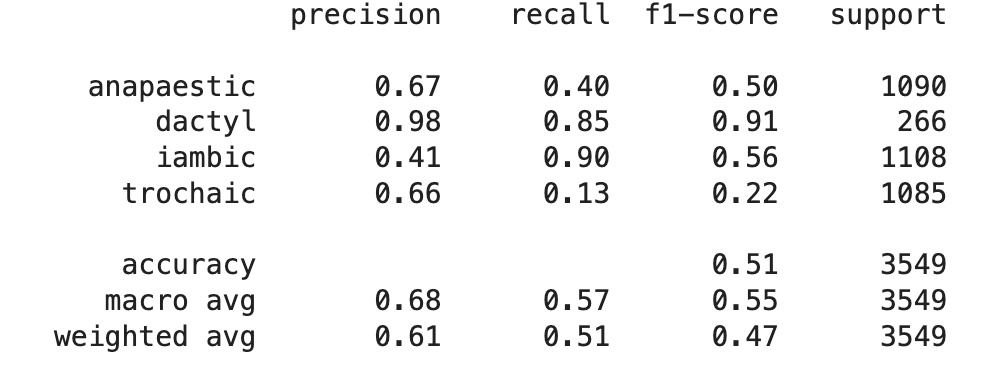
\includegraphics[width=0.9\linewidth, height=6cm]{images/con1D_af.png} 
\centering
\caption{Classification report}
\label{fig:addendum_cclass}
\end{subfigure}
    
\end{figure}
\end{document}
